\begin{figure}[ht]
\begin{center}
\begin{adjustbox}{width=0.7\textwidth}

    \tikzset{every picture/.style={line width=0.75pt}} %set default line width to 0.75pt        
    
    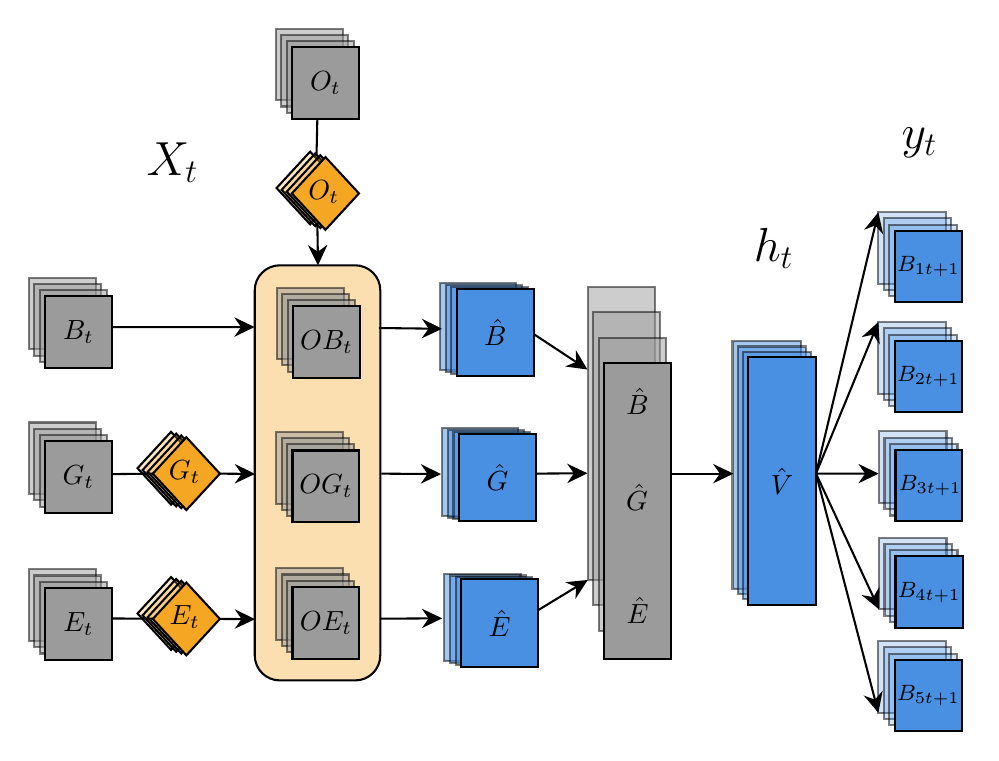
\begin{tikzpicture}[x=0.75pt,y=0.75pt,yscale=-1,xscale=1]
    %uncomment if require: \path (0,1033); %set diagram left start at 0, and has height of 1033
    
    %Rounded Rect [id:dp15650356150345013] 
    \draw  [fill={rgb, 255:red, 245; green, 166; blue, 35 }  ,fill opacity=0.36 ] (219.9,142.15) .. controls (219.9,135.47) and (225.32,130.05) .. (232,130.05) -- (268.3,130.05) .. controls (274.98,130.05) and (280.4,135.47) .. (280.4,142.15) -- (280.4,317.95) .. controls (280.4,324.63) and (274.98,330.05) .. (268.3,330.05) -- (232,330.05) .. controls (225.32,330.05) and (219.9,324.63) .. (219.9,317.95) -- cycle ;
    %Straight Lines [id:da409284418173784] 
    \draw    (250.06,109.76) -- (250.35,127.05) ;
    \draw [shift={(250.4,130.05)}, rotate = 269.03] [fill={rgb, 255:red, 0; green, 0; blue, 0 }  ][line width=0.08]  [draw opacity=0] (9.82,-4.72) -- (0,0) -- (9.82,4.72) -- (6.52,0) -- cycle    ;
    %Shape: Rectangle [id:dp7034345660290355] 
    \draw  [color={rgb, 255:red, 0; green, 0; blue, 0 }  ,draw opacity=0.5 ][fill={rgb, 255:red, 155; green, 155; blue, 155 }  ,fill opacity=0.5 ] (111.01,276.53) -- (143.26,276.53) -- (143.26,311.05) -- (111.01,311.05) -- cycle ;
    %Shape: Rectangle [id:dp22118233628007533] 
    \draw  [color={rgb, 255:red, 0; green, 0; blue, 0 }  ,draw opacity=0.5 ][fill={rgb, 255:red, 155; green, 155; blue, 155 }  ,fill opacity=0.5 ] (113.63,279.51) -- (145.88,279.51) -- (145.88,314.03) -- (113.63,314.03) -- cycle ;
    %Shape: Rectangle [id:dp24867768000931467] 
    \draw  [color={rgb, 255:red, 0; green, 0; blue, 0 }  ,draw opacity=0.5 ][fill={rgb, 255:red, 155; green, 155; blue, 155 }  ,fill opacity=0.5 ] (116.27,282.56) -- (148.53,282.56) -- (148.53,317.08) -- (116.27,317.08) -- cycle ;
    %Shape: Rectangle [id:dp124905579804508] 
    \draw  [fill={rgb, 255:red, 155; green, 155; blue, 155 }  ,fill opacity=1 ] (118.86,285.5) -- (151.11,285.5) -- (151.11,320.02) -- (118.86,320.02) -- cycle ;
    %Straight Lines [id:da8537240673366849] 
    \draw    (250.06,59.86) -- (249.67,77.43) ;
    %Shape: Rectangle [id:dp1958055080757597] 
    \draw  [color={rgb, 255:red, 0; green, 0; blue, 0 }  ,draw opacity=0.5 ][fill={rgb, 255:red, 74; green, 144; blue, 226 }  ,fill opacity=0.25 ] (520.36,157.39) -- (552.87,157.39) -- (552.87,191.9) -- (520.36,191.9) -- cycle ;
    %Shape: Rectangle [id:dp20825701586292622] 
    \draw  [color={rgb, 255:red, 0; green, 0; blue, 0 }  ,draw opacity=0.5 ][fill={rgb, 255:red, 74; green, 144; blue, 226 }  ,fill opacity=0.25 ] (523,160.37) -- (555.51,160.37) -- (555.51,194.88) -- (523,194.88) -- cycle ;
    %Shape: Rectangle [id:dp6709034910590727] 
    \draw  [color={rgb, 255:red, 0; green, 0; blue, 0 }  ,draw opacity=0.5 ][fill={rgb, 255:red, 74; green, 144; blue, 226 }  ,fill opacity=0.25 ] (525.67,163.42) -- (558.17,163.42) -- (558.17,197.93) -- (525.67,197.93) -- cycle ;
    %Shape: Rectangle [id:dp943426610209301] 
    \draw  [fill={rgb, 255:red, 74; green, 144; blue, 226 }  ,fill opacity=1 ] (528.28,166.36) -- (560.78,166.36) -- (560.78,200.87) -- (528.28,200.87) -- cycle ;
    %Shape: Rectangle [id:dp9270730461824767] 
    \draw  [color={rgb, 255:red, 0; green, 0; blue, 0 }  ,draw opacity=0.5 ][fill={rgb, 255:red, 74; green, 144; blue, 226 }  ,fill opacity=0.25 ] (520.69,210.06) -- (553.2,210.06) -- (553.2,244.56) -- (520.69,244.56) -- cycle ;
    %Shape: Rectangle [id:dp9671567967621458] 
    \draw  [color={rgb, 255:red, 0; green, 0; blue, 0 }  ,draw opacity=0.5 ][fill={rgb, 255:red, 74; green, 144; blue, 226 }  ,fill opacity=0.25 ] (523.33,213.04) -- (555.84,213.04) -- (555.84,247.54) -- (523.33,247.54) -- cycle ;
    %Shape: Rectangle [id:dp6567850092606636] 
    \draw  [color={rgb, 255:red, 0; green, 0; blue, 0 }  ,draw opacity=0.5 ][fill={rgb, 255:red, 74; green, 144; blue, 226 }  ,fill opacity=0.25 ] (526,216.09) -- (558.5,216.09) -- (558.5,250.6) -- (526,250.6) -- cycle ;
    %Shape: Rectangle [id:dp9307909660529495] 
    \draw  [fill={rgb, 255:red, 74; green, 144; blue, 226 }  ,fill opacity=1 ] (528.62,219.02) -- (560.84,219.02) -- (560.84,253.22) -- (528.62,253.22) -- cycle ;
    %Shape: Rectangle [id:dp2956426995252315] 
    \draw  [color={rgb, 255:red, 0; green, 0; blue, 0 }  ,draw opacity=0.5 ][fill={rgb, 255:red, 74; green, 144; blue, 226 }  ,fill opacity=0.25 ] (520.36,311.11) -- (552.87,311.11) -- (552.87,345.62) -- (520.36,345.62) -- cycle ;
    %Shape: Rectangle [id:dp9676718309145981] 
    \draw  [color={rgb, 255:red, 0; green, 0; blue, 0 }  ,draw opacity=0.5 ][fill={rgb, 255:red, 74; green, 144; blue, 226 }  ,fill opacity=0.25 ] (523,314.09) -- (555.51,314.09) -- (555.51,348.6) -- (523,348.6) -- cycle ;
    %Shape: Rectangle [id:dp3802447939611997] 
    \draw  [color={rgb, 255:red, 0; green, 0; blue, 0 }  ,draw opacity=0.5 ][fill={rgb, 255:red, 74; green, 144; blue, 226 }  ,fill opacity=0.25 ] (525.67,317.14) -- (558.17,317.14) -- (558.17,351.65) -- (525.67,351.65) -- cycle ;
    %Shape: Rectangle [id:dp2655409211543931] 
    \draw  [fill={rgb, 255:red, 74; green, 144; blue, 226 }  ,fill opacity=1 ] (528.28,320.08) -- (560.78,320.08) -- (560.78,354.59) -- (528.28,354.59) -- cycle ;
    %Shape: Rectangle [id:dp4040153422296009] 
    \draw  [color={rgb, 255:red, 0; green, 0; blue, 0 }  ,draw opacity=0.5 ][fill={rgb, 255:red, 74; green, 144; blue, 226 }  ,fill opacity=0.25 ] (520.69,261.32) -- (553.2,261.32) -- (553.2,295.83) -- (520.69,295.83) -- cycle ;
    %Shape: Rectangle [id:dp7066102537923638] 
    \draw  [color={rgb, 255:red, 0; green, 0; blue, 0 }  ,draw opacity=0.5 ][fill={rgb, 255:red, 74; green, 144; blue, 226 }  ,fill opacity=0.25 ] (523.33,264.3) -- (555.84,264.3) -- (555.84,298.81) -- (523.33,298.81) -- cycle ;
    %Shape: Rectangle [id:dp46050637304135866] 
    \draw  [color={rgb, 255:red, 0; green, 0; blue, 0 }  ,draw opacity=0.5 ][fill={rgb, 255:red, 74; green, 144; blue, 226 }  ,fill opacity=0.25 ] (526,267.35) -- (558.5,267.35) -- (558.5,301.86) -- (526,301.86) -- cycle ;
    %Shape: Rectangle [id:dp2033829273595421] 
    \draw  [fill={rgb, 255:red, 74; green, 144; blue, 226 }  ,fill opacity=1 ] (528.61,270.29) -- (561.11,270.29) -- (561.11,304.8) -- (528.61,304.8) -- cycle ;
    %Shape: Rectangle [id:dp19424752965877823] 
    \draw  [color={rgb, 255:red, 0; green, 0; blue, 0 }  ,draw opacity=0.5 ][fill={rgb, 255:red, 74; green, 144; blue, 226 }  ,fill opacity=0.25 ] (520.36,104.48) -- (552.87,104.48) -- (552.87,138.98) -- (520.36,138.98) -- cycle ;
    %Shape: Rectangle [id:dp6987771152166413] 
    \draw  [color={rgb, 255:red, 0; green, 0; blue, 0 }  ,draw opacity=0.5 ][fill={rgb, 255:red, 74; green, 144; blue, 226 }  ,fill opacity=0.25 ] (523,107.46) -- (555.51,107.46) -- (555.51,141.96) -- (523,141.96) -- cycle ;
    %Shape: Rectangle [id:dp12765942569283661] 
    \draw  [color={rgb, 255:red, 0; green, 0; blue, 0 }  ,draw opacity=0.5 ][fill={rgb, 255:red, 74; green, 144; blue, 226 }  ,fill opacity=0.25 ] (525.67,110.51) -- (558.17,110.51) -- (558.17,145.01) -- (525.67,145.01) -- cycle ;
    %Shape: Rectangle [id:dp16248810139444148] 
    \draw  [fill={rgb, 255:red, 74; green, 144; blue, 226 }  ,fill opacity=1 ] (528.28,113.44) -- (560.78,113.44) -- (560.78,147.95) -- (528.28,147.95) -- cycle ;
    %Shape: Rectangle [id:dp7988673729176894] 
    \draw  [color={rgb, 255:red, 0; green, 0; blue, 0 }  ,draw opacity=0.5 ][fill={rgb, 255:red, 155; green, 155; blue, 155 }  ,fill opacity=0.5 ] (111.01,205.77) -- (143.26,205.77) -- (143.26,240.29) -- (111.01,240.29) -- cycle ;
    %Shape: Rectangle [id:dp9623129937085917] 
    \draw  [color={rgb, 255:red, 0; green, 0; blue, 0 }  ,draw opacity=0.5 ][fill={rgb, 255:red, 155; green, 155; blue, 155 }  ,fill opacity=0.5 ] (113.63,208.75) -- (145.88,208.75) -- (145.88,243.27) -- (113.63,243.27) -- cycle ;
    %Shape: Rectangle [id:dp429379441325212] 
    \draw  [color={rgb, 255:red, 0; green, 0; blue, 0 }  ,draw opacity=0.5 ][fill={rgb, 255:red, 155; green, 155; blue, 155 }  ,fill opacity=0.5 ] (116.27,211.8) -- (148.53,211.8) -- (148.53,246.32) -- (116.27,246.32) -- cycle ;
    %Shape: Rectangle [id:dp9493890675957639] 
    \draw  [fill={rgb, 255:red, 155; green, 155; blue, 155 }  ,fill opacity=1 ] (118.86,214.74) -- (151.11,214.74) -- (151.11,249.26) -- (118.86,249.26) -- cycle ;
    %Straight Lines [id:da0399560958706785] 
    \draw [fill={rgb, 255:red, 155; green, 155; blue, 155 }  ,fill opacity=1 ]   (150.09,159.83) -- (216.85,159.8) ;
    \draw [shift={(219.85,159.8)}, rotate = 179.98] [fill={rgb, 255:red, 0; green, 0; blue, 0 }  ][line width=0.08]  [draw opacity=0] (9.82,-4.72) -- (0,0) -- (9.82,4.72) -- (6.52,0) -- cycle    ;
    %Shape: Rectangle [id:dp3393145890474042] 
    \draw  [color={rgb, 255:red, 0; green, 0; blue, 0 }  ,draw opacity=0.5 ][fill={rgb, 255:red, 155; green, 155; blue, 155 }  ,fill opacity=0.5 ] (111.01,136.06) -- (143.26,136.06) -- (143.26,170.57) -- (111.01,170.57) -- cycle ;
    %Shape: Rectangle [id:dp27631704382885136] 
    \draw  [color={rgb, 255:red, 0; green, 0; blue, 0 }  ,draw opacity=0.5 ][fill={rgb, 255:red, 155; green, 155; blue, 155 }  ,fill opacity=0.5 ] (113.63,139.04) -- (145.88,139.04) -- (145.88,173.55) -- (113.63,173.55) -- cycle ;
    %Shape: Rectangle [id:dp8553441662393909] 
    \draw  [color={rgb, 255:red, 0; green, 0; blue, 0 }  ,draw opacity=0.5 ][fill={rgb, 255:red, 155; green, 155; blue, 155 }  ,fill opacity=0.5 ] (116.27,142.09) -- (148.53,142.09) -- (148.53,176.61) -- (116.27,176.61) -- cycle ;
    %Shape: Rectangle [id:dp4571491350911555] 
    \draw  [fill={rgb, 255:red, 155; green, 155; blue, 155 }  ,fill opacity=1 ] (118.86,145.03) -- (151.11,145.03) -- (151.11,179.54) -- (118.86,179.54) -- cycle ;
    %Shape: Diamond [id:dp42134346339770745] 
    \draw  [fill={rgb, 255:red, 245; green, 166; blue, 35 }  ,fill opacity=0.25 ] (179.6,210.28) -- (195.77,227.81) -- (179.6,245.33) -- (163.43,227.81) -- cycle ;
    %Shape: Diamond [id:dp8160874162123375] 
    \draw  [fill={rgb, 255:red, 245; green, 166; blue, 35 }  ,fill opacity=0.25 ] (182.05,211.16) -- (198.22,228.68) -- (182.05,246.2) -- (165.89,228.68) -- cycle ;
    %Shape: Diamond [id:dp05986250472128074] 
    \draw  [fill={rgb, 255:red, 245; green, 166; blue, 35 }  ,fill opacity=0.25 ] (184.51,212.04) -- (200.68,229.56) -- (184.51,247.08) -- (168.34,229.56) -- cycle ;
    %Shape: Diamond [id:dp6831575900746938] 
    \draw  [fill={rgb, 255:red, 245; green, 166; blue, 35 }  ,fill opacity=1 ] (186.97,212.91) -- (203.13,230.43) -- (186.97,247.96) -- (170.8,230.43) -- cycle ;
    %Straight Lines [id:da3169233008507637] 
    \draw    (151.46,230.66) -- (170.8,230.43) ;
    %Shape: Diamond [id:dp08100159339963764] 
    \draw  [fill={rgb, 255:red, 245; green, 166; blue, 35 }  ,fill opacity=0.25 ] (179.6,280.28) -- (195.77,297.81) -- (179.6,315.33) -- (163.43,297.81) -- cycle ;
    %Shape: Diamond [id:dp6545409040088919] 
    \draw  [fill={rgb, 255:red, 245; green, 166; blue, 35 }  ,fill opacity=0.25 ] (182.05,281.16) -- (198.22,298.68) -- (182.05,316.2) -- (165.89,298.68) -- cycle ;
    %Shape: Diamond [id:dp22008618792927115] 
    \draw  [fill={rgb, 255:red, 245; green, 166; blue, 35 }  ,fill opacity=0.25 ] (184.51,282.04) -- (200.68,299.56) -- (184.51,317.08) -- (168.34,299.56) -- cycle ;
    %Shape: Diamond [id:dp6216162169932065] 
    \draw  [fill={rgb, 255:red, 245; green, 166; blue, 35 }  ,fill opacity=1 ] (186.97,282.91) -- (203.13,300.43) -- (186.97,317.96) -- (170.8,300.43) -- cycle ;
    %Straight Lines [id:da6348314705630924] 
    \draw    (203.13,300.43) -- (217.07,300.51) ;
    \draw [shift={(220.07,300.53)}, rotate = 180.32] [fill={rgb, 255:red, 0; green, 0; blue, 0 }  ][line width=0.08]  [draw opacity=0] (9.82,-4.72) -- (0,0) -- (9.82,4.72) -- (6.52,0) -- cycle    ;
    %Straight Lines [id:da29443986089740126] 
    \draw    (150.89,300.2) -- (170.89,300.31) ;
    %Straight Lines [id:da7037674707293678] 
    \draw [fill={rgb, 255:red, 155; green, 155; blue, 155 }  ,fill opacity=1 ]   (279.77,160.26) -- (307.2,160.6) ;
    \draw [shift={(310.2,160.63)}, rotate = 180.71] [fill={rgb, 255:red, 0; green, 0; blue, 0 }  ][line width=0.08]  [draw opacity=0] (9.82,-4.72) -- (0,0) -- (9.82,4.72) -- (6.52,0) -- cycle    ;
    %Straight Lines [id:da04725287763752273] 
    \draw [fill={rgb, 255:red, 155; green, 155; blue, 155 }  ,fill opacity=1 ]   (350.2,160.45) -- (377.7,178.6) ;
    \draw [shift={(380.2,180.25)}, rotate = 213.42] [fill={rgb, 255:red, 0; green, 0; blue, 0 }  ][line width=0.08]  [draw opacity=0] (9.82,-4.72) -- (0,0) -- (9.82,4.72) -- (6.52,0) -- cycle    ;
    %Straight Lines [id:da6945773359077246] 
    \draw    (203.13,230.43) -- (217.07,230.54) ;
    \draw [shift={(220.07,230.56)}, rotate = 180.44] [fill={rgb, 255:red, 0; green, 0; blue, 0 }  ][line width=0.08]  [draw opacity=0] (9.82,-4.72) -- (0,0) -- (9.82,4.72) -- (6.52,0) -- cycle    ;
    %Straight Lines [id:da6273046628189572] 
    \draw [fill={rgb, 255:red, 155; green, 155; blue, 155 }  ,fill opacity=1 ]   (280.91,230.43) -- (306.7,230.61) ;
    \draw [shift={(309.7,230.63)}, rotate = 180.41] [fill={rgb, 255:red, 0; green, 0; blue, 0 }  ][line width=0.08]  [draw opacity=0] (9.82,-4.72) -- (0,0) -- (9.82,4.72) -- (6.52,0) -- cycle    ;
    %Straight Lines [id:da5724582303552335] 
    \draw [fill={rgb, 255:red, 155; green, 155; blue, 155 }  ,fill opacity=1 ]   (280.63,300.31) -- (307.2,300.15) ;
    \draw [shift={(310.2,300.13)}, rotate = 179.65] [fill={rgb, 255:red, 0; green, 0; blue, 0 }  ][line width=0.08]  [draw opacity=0] (9.82,-4.72) -- (0,0) -- (9.82,4.72) -- (6.52,0) -- cycle    ;
    %Shape: Rectangle [id:dp53907172122875] 
    \draw  [color={rgb, 255:red, 0; green, 0; blue, 0 }  ,draw opacity=0.5 ][fill={rgb, 255:red, 155; green, 155; blue, 155 }  ,fill opacity=0.5 ] (230.01,16.06) -- (262.26,16.06) -- (262.26,50.57) -- (230.01,50.57) -- cycle ;
    %Shape: Rectangle [id:dp009192212091793661] 
    \draw  [color={rgb, 255:red, 0; green, 0; blue, 0 }  ,draw opacity=0.5 ][fill={rgb, 255:red, 155; green, 155; blue, 155 }  ,fill opacity=0.5 ] (232.63,19.04) -- (264.88,19.04) -- (264.88,53.55) -- (232.63,53.55) -- cycle ;
    %Shape: Rectangle [id:dp10982806096562447] 
    \draw  [color={rgb, 255:red, 0; green, 0; blue, 0 }  ,draw opacity=0.5 ][fill={rgb, 255:red, 155; green, 155; blue, 155 }  ,fill opacity=0.5 ] (235.27,22.09) -- (267.53,22.09) -- (267.53,56.61) -- (235.27,56.61) -- cycle ;
    %Shape: Rectangle [id:dp024787601372134982] 
    \draw  [fill={rgb, 255:red, 155; green, 155; blue, 155 }  ,fill opacity=1 ] (237.86,25.03) -- (270.11,25.03) -- (270.11,59.54) -- (237.86,59.54) -- cycle ;
    %Shape: Rectangle [id:dp9022114030928725] 
    \draw  [color={rgb, 255:red, 0; green, 0; blue, 0 }  ,draw opacity=0.5 ][fill={rgb, 255:red, 155; green, 155; blue, 155 }  ,fill opacity=0.5 ] (380.34,140.45) -- (412.6,140.45) -- (412.6,281.66) -- (380.34,281.66) -- cycle ;
    %Shape: Rectangle [id:dp9877830883323443] 
    \draw  [color={rgb, 255:red, 0; green, 0; blue, 0 }  ,draw opacity=0.5 ][fill={rgb, 255:red, 155; green, 155; blue, 155 }  ,fill opacity=0.5 ] (382.96,152.64) -- (415.22,152.64) -- (415.22,293.84) -- (382.96,293.84) -- cycle ;
    %Shape: Rectangle [id:dp8814167498359042] 
    \draw  [color={rgb, 255:red, 0; green, 0; blue, 0 }  ,draw opacity=0.5 ][fill={rgb, 255:red, 155; green, 155; blue, 155 }  ,fill opacity=0.5 ] (385.61,165.13) -- (417.86,165.13) -- (417.86,306.34) -- (385.61,306.34) -- cycle ;
    %Shape: Rectangle [id:dp5289911737134959] 
    \draw  [fill={rgb, 255:red, 155; green, 155; blue, 155 }  ,fill opacity=1 ] (388.19,177.14) -- (420.45,177.14) -- (420.45,319.53) -- (388.19,319.53) -- cycle ;
    %Shape: Rectangle [id:dp8149328215662492] 
    \draw  [color={rgb, 255:red, 0; green, 0; blue, 0 }  ,draw opacity=0.5 ][fill={rgb, 255:red, 155; green, 155; blue, 155 }  ,fill opacity=0.5 ] (230.51,140.77) -- (262.76,140.77) -- (262.76,175.29) -- (230.51,175.29) -- cycle ;
    %Shape: Rectangle [id:dp45921305478843055] 
    \draw  [color={rgb, 255:red, 0; green, 0; blue, 0 }  ,draw opacity=0.5 ][fill={rgb, 255:red, 155; green, 155; blue, 155 }  ,fill opacity=0.5 ] (233.13,143.75) -- (265.38,143.75) -- (265.38,178.27) -- (233.13,178.27) -- cycle ;
    %Shape: Rectangle [id:dp6228279530655318] 
    \draw  [color={rgb, 255:red, 0; green, 0; blue, 0 }  ,draw opacity=0.5 ][fill={rgb, 255:red, 155; green, 155; blue, 155 }  ,fill opacity=0.5 ] (235.77,146.8) -- (268.03,146.8) -- (268.03,181.32) -- (235.77,181.32) -- cycle ;
    %Shape: Rectangle [id:dp3598797805540589] 
    \draw  [fill={rgb, 255:red, 155; green, 155; blue, 155 }  ,fill opacity=1 ] (238.36,149.74) -- (270.61,149.74) -- (270.61,184.26) -- (238.36,184.26) -- cycle ;
    %Shape: Rectangle [id:dp9661891091990619] 
    \draw  [color={rgb, 255:red, 0; green, 0; blue, 0 }  ,draw opacity=0.5 ][fill={rgb, 255:red, 155; green, 155; blue, 155 }  ,fill opacity=0.5 ] (230.26,210.32) -- (262.51,210.32) -- (262.51,244.84) -- (230.26,244.84) -- cycle ;
    %Shape: Rectangle [id:dp690231151268716] 
    \draw  [color={rgb, 255:red, 0; green, 0; blue, 0 }  ,draw opacity=0.5 ][fill={rgb, 255:red, 155; green, 155; blue, 155 }  ,fill opacity=0.5 ] (232.88,213.3) -- (265.13,213.3) -- (265.13,247.82) -- (232.88,247.82) -- cycle ;
    %Shape: Rectangle [id:dp48804619093484347] 
    \draw  [color={rgb, 255:red, 0; green, 0; blue, 0 }  ,draw opacity=0.5 ][fill={rgb, 255:red, 155; green, 155; blue, 155 }  ,fill opacity=0.5 ] (235.52,216.35) -- (267.78,216.35) -- (267.78,250.87) -- (235.52,250.87) -- cycle ;
    %Shape: Rectangle [id:dp22992925838286216] 
    \draw  [fill={rgb, 255:red, 155; green, 155; blue, 155 }  ,fill opacity=1 ] (238.11,219.29) -- (270.36,219.29) -- (270.36,253.81) -- (238.11,253.81) -- cycle ;
    %Shape: Rectangle [id:dp29039742489844134] 
    \draw  [color={rgb, 255:red, 0; green, 0; blue, 0 }  ,draw opacity=0.5 ][fill={rgb, 255:red, 155; green, 155; blue, 155 }  ,fill opacity=0.5 ] (230.26,276.02) -- (262.51,276.02) -- (262.51,310.54) -- (230.26,310.54) -- cycle ;
    %Shape: Rectangle [id:dp42091335353816794] 
    \draw  [color={rgb, 255:red, 0; green, 0; blue, 0 }  ,draw opacity=0.5 ][fill={rgb, 255:red, 155; green, 155; blue, 155 }  ,fill opacity=0.5 ] (232.88,279) -- (265.13,279) -- (265.13,313.52) -- (232.88,313.52) -- cycle ;
    %Shape: Rectangle [id:dp9855473947081604] 
    \draw  [color={rgb, 255:red, 0; green, 0; blue, 0 }  ,draw opacity=0.5 ][fill={rgb, 255:red, 155; green, 155; blue, 155 }  ,fill opacity=0.5 ] (235.52,282.05) -- (267.78,282.05) -- (267.78,316.57) -- (235.52,316.57) -- cycle ;
    %Shape: Rectangle [id:dp434232717458334] 
    \draw  [fill={rgb, 255:red, 155; green, 155; blue, 155 }  ,fill opacity=1 ] (238.11,284.99) -- (270.36,284.99) -- (270.36,319.51) -- (238.11,319.51) -- cycle ;
    %Shape: Diamond [id:dp30872576312410427] 
    \draw  [fill={rgb, 255:red, 245; green, 166; blue, 35 }  ,fill opacity=0.25 ] (246.6,75.28) -- (262.77,92.81) -- (246.6,110.33) -- (230.43,92.81) -- cycle ;
    %Shape: Diamond [id:dp6849972388912634] 
    \draw  [fill={rgb, 255:red, 245; green, 166; blue, 35 }  ,fill opacity=0.25 ] (249.05,76.16) -- (265.22,93.68) -- (249.05,111.2) -- (232.89,93.68) -- cycle ;
    %Shape: Diamond [id:dp857485897511279] 
    \draw  [fill={rgb, 255:red, 245; green, 166; blue, 35 }  ,fill opacity=0.25 ] (251.51,77.04) -- (267.68,94.56) -- (251.51,112.08) -- (235.34,94.56) -- cycle ;
    %Shape: Diamond [id:dp49326046176048577] 
    \draw  [fill={rgb, 255:red, 245; green, 166; blue, 35 }  ,fill opacity=1 ] (253.97,77.91) -- (270.13,95.43) -- (253.97,112.96) -- (237.8,95.43) -- cycle ;
    %Straight Lines [id:da9533396825264671] 
    \draw [fill={rgb, 255:red, 155; green, 155; blue, 155 }  ,fill opacity=1 ]   (349.2,230.45) -- (377.2,230.27) ;
    \draw [shift={(380.2,230.25)}, rotate = 179.63] [fill={rgb, 255:red, 0; green, 0; blue, 0 }  ][line width=0.08]  [draw opacity=0] (9.82,-4.72) -- (0,0) -- (9.82,4.72) -- (6.52,0) -- cycle    ;
    %Straight Lines [id:da46693829157920863] 
    \draw [fill={rgb, 255:red, 155; green, 155; blue, 155 }  ,fill opacity=1 ]   (350.4,299.88) -- (377.78,283.22) ;
    \draw [shift={(380.34,281.66)}, rotate = 148.68] [fill={rgb, 255:red, 0; green, 0; blue, 0 }  ][line width=0.08]  [draw opacity=0] (9.82,-4.72) -- (0,0) -- (9.82,4.72) -- (6.52,0) -- cycle    ;
    %Straight Lines [id:da9477168442608538] 
    \draw [fill={rgb, 255:red, 155; green, 155; blue, 155 }  ,fill opacity=1 ]   (421.09,230.43) -- (447.51,230.43) ;
    \draw [shift={(450.51,230.43)}, rotate = 180] [fill={rgb, 255:red, 0; green, 0; blue, 0 }  ][line width=0.08]  [draw opacity=0] (9.82,-4.72) -- (0,0) -- (9.82,4.72) -- (6.52,0) -- cycle    ;
    %Straight Lines [id:da17588566125157779] 
    \draw [fill={rgb, 255:red, 155; green, 155; blue, 155 }  ,fill opacity=1 ]   (490.32,230.39) -- (517.51,230.42) ;
    \draw [shift={(520.51,230.43)}, rotate = 180.08] [fill={rgb, 255:red, 0; green, 0; blue, 0 }  ][line width=0.08]  [draw opacity=0] (9.82,-4.72) -- (0,0) -- (9.82,4.72) -- (6.52,0) -- cycle    ;
    %Straight Lines [id:da990575471229112] 
    \draw [fill={rgb, 255:red, 155; green, 155; blue, 155 }  ,fill opacity=1 ]   (490.32,230.39) -- (519.43,293.11) ;
    \draw [shift={(520.69,295.83)}, rotate = 245.1] [fill={rgb, 255:red, 0; green, 0; blue, 0 }  ][line width=0.08]  [draw opacity=0] (9.82,-4.72) -- (0,0) -- (9.82,4.72) -- (6.52,0) -- cycle    ;
    %Straight Lines [id:da11726542356327818] 
    \draw [fill={rgb, 255:red, 155; green, 155; blue, 155 }  ,fill opacity=1 ]   (490.32,230.39) -- (519.61,342.72) ;
    \draw [shift={(520.36,345.62)}, rotate = 255.39] [fill={rgb, 255:red, 0; green, 0; blue, 0 }  ][line width=0.08]  [draw opacity=0] (9.82,-4.72) -- (0,0) -- (9.82,4.72) -- (6.52,0) -- cycle    ;
    %Straight Lines [id:da6006783627611112] 
    \draw [fill={rgb, 255:red, 155; green, 155; blue, 155 }  ,fill opacity=1 ]   (490.32,230.39) -- (519.22,160.17) ;
    \draw [shift={(520.36,157.39)}, rotate = 112.37] [fill={rgb, 255:red, 0; green, 0; blue, 0 }  ][line width=0.08]  [draw opacity=0] (9.82,-4.72) -- (0,0) -- (9.82,4.72) -- (6.52,0) -- cycle    ;
    %Straight Lines [id:da16067428057688105] 
    \draw [fill={rgb, 255:red, 155; green, 155; blue, 155 }  ,fill opacity=1 ]   (490.32,230.39) -- (519.67,107.4) ;
    \draw [shift={(520.36,104.48)}, rotate = 103.42] [fill={rgb, 255:red, 0; green, 0; blue, 0 }  ][line width=0.08]  [draw opacity=0] (9.82,-4.72) -- (0,0) -- (9.82,4.72) -- (6.52,0) -- cycle    ;
    %Shape: Rectangle [id:dp04777231109494484] 
    \draw  [color={rgb, 255:red, 0; green, 0; blue, 0 }  ,draw opacity=0.5 ][fill={rgb, 255:red, 74; green, 144; blue, 226 }  ,fill opacity=0.5 ] (309.1,138.6) -- (345.95,138.6) -- (345.95,180.65) -- (309.1,180.65) -- cycle ;
    %Shape: Rectangle [id:dp7558311796324689] 
    \draw  [color={rgb, 255:red, 0; green, 0; blue, 0 }  ,draw opacity=0.5 ][fill={rgb, 255:red, 74; green, 144; blue, 226 }  ,fill opacity=0.5 ] (311.88,139.51) -- (348.73,139.51) -- (348.73,181.56) -- (311.88,181.56) -- cycle ;
    %Shape: Rectangle [id:dp02297715036875614] 
    \draw  [color={rgb, 255:red, 0; green, 0; blue, 0 }  ,draw opacity=0.5 ][fill={rgb, 255:red, 74; green, 144; blue, 226 }  ,fill opacity=0.5 ] (314.67,140.42) -- (351.51,140.42) -- (351.51,182.46) -- (314.67,182.46) -- cycle ;
    %Shape: Rectangle [id:dp7483619990673073] 
    \draw  [fill={rgb, 255:red, 74; green, 144; blue, 226 }  ,fill opacity=1 ] (317.45,141.33) -- (354.29,141.33) -- (354.29,183.37) -- (317.45,183.37) -- cycle ;
    %Shape: Rectangle [id:dp8163589302848298] 
    \draw  [color={rgb, 255:red, 0; green, 0; blue, 0 }  ,draw opacity=0.5 ][fill={rgb, 255:red, 74; green, 144; blue, 226 }  ,fill opacity=0.5 ] (450.1,166.6) -- (482.87,166.6) -- (482.87,285.87) -- (450.1,285.87) -- cycle ;
    %Shape: Rectangle [id:dp13561622734198409] 
    \draw  [color={rgb, 255:red, 0; green, 0; blue, 0 }  ,draw opacity=0.5 ][fill={rgb, 255:red, 74; green, 144; blue, 226 }  ,fill opacity=0.5 ] (452.57,169.18) -- (485.34,169.18) -- (485.34,288.44) -- (452.57,288.44) -- cycle ;
    %Shape: Rectangle [id:dp028266783786446537] 
    \draw  [color={rgb, 255:red, 0; green, 0; blue, 0 }  ,draw opacity=0.5 ][fill={rgb, 255:red, 74; green, 144; blue, 226 }  ,fill opacity=0.5 ] (455.05,171.76) -- (487.82,171.76) -- (487.82,291.02) -- (455.05,291.02) -- cycle ;
    %Shape: Rectangle [id:dp501556684499422] 
    \draw  [fill={rgb, 255:red, 74; green, 144; blue, 226 }  ,fill opacity=1 ] (457.52,174.33) -- (490.29,174.33) -- (490.29,293.6) -- (457.52,293.6) -- cycle ;
    
    %Shape: Rectangle [id:dp3431119253458095] 
    \draw  [color={rgb, 255:red, 0; green, 0; blue, 0 }  ,draw opacity=0.5 ][fill={rgb, 255:red, 74; green, 144; blue, 226 }  ,fill opacity=0.5 ] (310.1,208.6) -- (346.95,208.6) -- (346.95,250.65) -- (310.1,250.65) -- cycle ;
    %Shape: Rectangle [id:dp8294825257941912] 
    \draw  [color={rgb, 255:red, 0; green, 0; blue, 0 }  ,draw opacity=0.5 ][fill={rgb, 255:red, 74; green, 144; blue, 226 }  ,fill opacity=0.5 ] (312.88,209.51) -- (349.73,209.51) -- (349.73,251.56) -- (312.88,251.56) -- cycle ;
    %Shape: Rectangle [id:dp049289680132614255] 
    \draw  [color={rgb, 255:red, 0; green, 0; blue, 0 }  ,draw opacity=0.5 ][fill={rgb, 255:red, 74; green, 144; blue, 226 }  ,fill opacity=0.5 ] (315.67,210.42) -- (352.51,210.42) -- (352.51,252.46) -- (315.67,252.46) -- cycle ;
    %Shape: Rectangle [id:dp4657902939703581] 
    \draw  [fill={rgb, 255:red, 74; green, 144; blue, 226 }  ,fill opacity=1 ] (318.45,211.33) -- (355.29,211.33) -- (355.29,253.37) -- (318.45,253.37) -- cycle ;
    %Shape: Rectangle [id:dp8549615376830864] 
    \draw  [color={rgb, 255:red, 0; green, 0; blue, 0 }  ,draw opacity=0.5 ][fill={rgb, 255:red, 74; green, 144; blue, 226 }  ,fill opacity=0.5 ] (311.1,278.6) -- (347.95,278.6) -- (347.95,320.65) -- (311.1,320.65) -- cycle ;
    %Shape: Rectangle [id:dp07757251126817089] 
    \draw  [color={rgb, 255:red, 0; green, 0; blue, 0 }  ,draw opacity=0.5 ][fill={rgb, 255:red, 74; green, 144; blue, 226 }  ,fill opacity=0.5 ] (313.88,279.51) -- (350.73,279.51) -- (350.73,321.56) -- (313.88,321.56) -- cycle ;
    %Shape: Rectangle [id:dp9077595517238054] 
    \draw  [color={rgb, 255:red, 0; green, 0; blue, 0 }  ,draw opacity=0.5 ][fill={rgb, 255:red, 74; green, 144; blue, 226 }  ,fill opacity=0.5 ] (316.67,280.42) -- (353.51,280.42) -- (353.51,322.46) -- (316.67,322.46) -- cycle ;
    %Shape: Rectangle [id:dp2039123260975314] 
    \draw  [fill={rgb, 255:red, 74; green, 144; blue, 226 }  ,fill opacity=1 ] (319.45,281.33) -- (356.29,281.33) -- (356.29,323.37) -- (319.45,323.37) -- cycle ;
    
    % Text Node
    \draw (134.99,302.76) node  [font=\normalsize]  {$E_{t}$};
    % Text Node
    \draw (180.34,80.58) node  [font=\LARGE]  {$X_{t}$};
    % Text Node
    \draw (470.01,121.94) node  [font=\LARGE]  {$h_{t}$};
    % Text Node
    \draw (544.53,183.61) node  [font=\footnotesize]  {$B_{2t+1}$};
    % Text Node
    \draw (545.41,236.28) node  [font=\footnotesize]  {$B_{3t+1}$};
    % Text Node
    \draw (544.86,287.54) node  [font=\footnotesize]  {$B_{4t+1}$};
    % Text Node
    \draw (544.53,337.33) node  [font=\footnotesize]  {$B_{5t+1}$};
    % Text Node
    \draw (540.21,70.84) node  [font=\LARGE]  {$y_{t}$};
    % Text Node
    \draw (544.53,130.7) node  [font=\footnotesize]  {$B_{1t+1}$};
    % Text Node
    \draw (134.99,232) node  [font=\normalsize]  {$G_{t}$};
    % Text Node
    \draw (134.99,162.29) node  [font=\normalsize]  {$B_{t}$};
    % Text Node
    \draw (186.15,229.56) node  [font=\normalsize]  {$G_{t}$};
    % Text Node
    \draw (186.15,299.56) node  [font=\normalsize]  {$E_{t}$};
    % Text Node
    \draw (253.99,42.29) node  [font=\normalsize]  {$O_{t}$};
    % Text Node
    \draw (254.49,167) node  [font=\normalsize]  {$OB_{t}$};
    % Text Node
    \draw (254.24,236.55) node  [font=\normalsize]  {$OG_{t}$};
    % Text Node
    \draw (254.24,302.25) node  [font=\normalsize]  {$OE_{t}$};
    % Text Node
    \draw (253.15,94.56) node  [font=\normalsize]  {$O_{t}$};
    % Text Node
    \draw (404.35,195.78) node  [font=\normalsize]  {$\hat{B}$};
    % Text Node
    \draw (404.07,242.06) node  [font=\normalsize]  {$\hat{G}$};
    % Text Node
    \draw (404.35,296.11) node  [font=\normalsize]  {$\hat{E}$};
    % Text Node
    \draw (473.91,233.97) node  [font=\normalsize]  {$\hat{V}$};
    % Text Node
    \draw (335.87,162.35) node  [font=\normalsize]  {$\hat{B}$};
    % Text Node
    \draw (336.87,232.35) node  [font=\normalsize]  {$\hat{G}$};
    % Text Node
    \draw (337.87,302.35) node  [font=\normalsize]  {$\hat{E}$};
    
    
    \end{tikzpicture}



\end{adjustbox}
\end{center}
\caption[\textbf{The environment-event time distributed multi layer perceptron architecture}]{Blue and orange shapes represent respectively feedforward and embedding operations. Gray shapes indicate operations with no learnable parameters, such as tensor instantiation and concatenation. Stacked, transparent colouring indicates tensors with a sequential structure. Straight arrows refer to the presence of feed-forward information flow. All the feedforward operations are time distributed.}
\label{fig: mlp_3}
\end{figure}